\chapter{Problem Definition} % Main chapter title

\label{Chapter:ProblemDefinitionandMotivation}

Carbon nano-materials are subjected to great interest for research purposes due to their various potential applications in diverse areas that take advantage of the nano-scale properties \cite{Siddiqui2019}. Carbon nano-materials are suitable for the catalysis, adsorption, carbon capture, energy and hydrogen storage, drug delivery, bio-sensing and cancer detection \cite{Siddiqui2019}. Some matchless properties that allow carbon nano-materials to be utilized within multiple functionalities include high porosity, distinguished structures, uniform morphologies, high stability, high magnetic properties and high conductivity \cite{Siddiqui2019}.

This document bestow a thesis proposal to perform a research to engineer and design a polymer solution to achieve mass scale manufacturing of high conductive carbon nano-wires with a reduced diameter in an inexpensive, continuous, simple and reproducible manner. The research intends to involve several manufacturing processes such as near field electrospinning, photopolymerization, pyrolization and carbonization, as they have shown to be promising methods for the fabrication of carbon nano-materials \cite{Cardenas2017}. See Figure \ref{fig:fabricationFlowChart}. A number of processes have been developed for specific purposes of polymeric nano-fibers, some include surface deposition, composites, and chemical adjustments. Polymeric nano-fibers must be also pyrolyzed to generate carbon nano-wires with conductive capabilities \cite{Madou2011} for electrochemical sensing and energy storage purposes.

\begin{figure}[th]
\centering
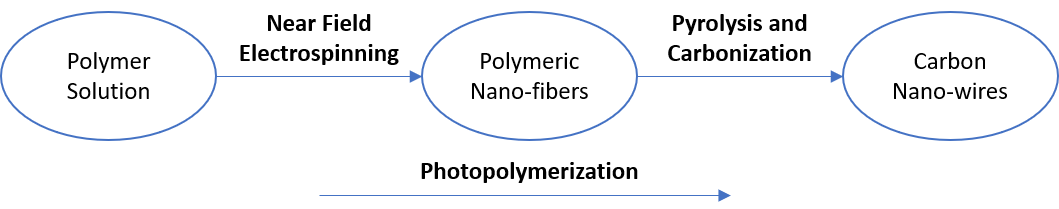
\includegraphics[width=0.95\textwidth]{./Figures/FabricationProcess.png}
\decoRule
\caption[Carbon Nano-wires Fabrication Process]{Fabrication process of carbon nano-wires to achieve through the proposed dissertation.}
\label{fig:fabricationFlowChart}
\end{figure}

Nanotechnology has explored different polymer patterning techniques to integrate carbon nano-wires structures. One technique is known as far-field electrospinning, a process in which electrified jets of polymer solution are dispensed to synthesize nano-fibers which then are pyrolyzed at high temperatures. One sub-technique derived from electrospinning is near field electromechanical spinning or EMS. EMS has proved to deliver high control in patterning polymeric nano-fibers \cite{Cardenas2017}.

The proposal is to continue the previous work done in regards of the synthesis of carbon nano-wires. Previous work includes the fabrication of suspended carbon nano-wires by two methods: electro-mechanical spinning and multiple-photon polymerization with a photoresist \cite{Cardenas2017}. This research proposal is intended to focus on electro-mechanical spinning processes only, to bring off polymer solutions that can be electrospun by near field electrospinning (NFES), photopolymerized and pyrolyzed into conducting carbon nano-wires. The polymer solutions described in Cardenas' work \cite{Cardenas2017} are to be amended to achieve the goal mentioned in the previous statement.

Traditional near-field electrospinning or NFES allows large scale manufacturability combined with controlled guidance \cite{Madou2011}. However, the reported efforts required the use of electric fields in excess of 200 kV/m for continuous operation, resulting in limited control for nano-fiber patterning in traditional NFES processes \cite{Madou2011}. The current state-of-the-art synthesis processes for polymer nano-fibers lack to yield precise, inexpensive, fast, and continuous manufacturing properties.

Carbon nanowires have been fabricated with a photoresist by multiple-photon polymerization techniques. However little is known about polymers that can produce conductive carbon nano-wires after pyrolysis. The lack of research relays on the fact that in the past years, it was assumed that most polymers are non-graphitic through pyrolysis \cite{Franklin1951}. In the past years photon polymerization processes have been applied to the fabrication of nano-structures with the use of a epoxy based photoresist \cite{Boer2014}. Photon polymerization techniques deliver patterning resolutions with nano-scale tolerances for the production of highly detailed structures \cite{Hribar2014}.

On the other hand, electrospinning has been acknowledged as a process with promising results at nano-structure fabrication \cite{Boer2014}, yet there is little research regarding the implementation of electrospinning for the fabrication of carbon nano-wires. Electrospinning has the potential to be a more straightforward process for the design and fabrication of nano-structures, as it can achieve mass scale manufacturing in a continuous, simple and reproducible manner. Cardenas \cite{Cardenas2017} shows that electrospinning can be implemented with ease for carbon nano-wire synthesis. Mechano-electrospinning, a new variant of electrospinning shows promising results in the production of ordered carbon nano-wires. As Cardenas states \cite{Cardenas2017}, mechano-electrospinning is an early technology invention, and brings new challenges, such as the reproducibility of carbon nano-wire production. Furthermore, the study of a new fabrication process to produce carbon nanowires that involves mechano-electrospinning will enable spatial control of the structures' patterning.

Since electrospinning seems to be a better alternative for carbon nano-wire fabrication processes; and for that purpose of its implementation, it is required to develop polymer solutions that can be mechano-electrospun, photopolymerized and pyrolyzed into conducting carbon nano-wires. Carbon nano-materials have been subjected to research due to their various potential applications in diverse areas that take advantage of the nano-scale properties \cite{Siddiqui2019}. Carbon nano-materials are suitable for the catalysis, adsorption, carbon capture, energy and hydrogen storage, drug delivery, bio-sensing and cancer detection \cite{Siddiqui2019}. However most applications are not currently feasible due to the lack of a continuous, simple and reproducible fabrication method with inexpensive processes. With the newly designed polymer solution, it would be possible to produce carbon nano-wires in large quantities, and therefore more applications will become feasible. On the other hand, the new technique will overcome some limitations of other methods such as lithography currently has. For instance, patterns created by lithography processes cannot be originated, only replicated, all constituent points of the pattern can only be addressed at the same time, and the process requires the pattern to be encoded into a mask \cite{Landis2011}.

In summary, the purpose of the proposed dissertation is to study the practice and feasibility of a new fabrication process to achieve mass scale manufacturing of carbon nano-wires in an inexpensive, continuous, simple and reproducible manner; by the integration of mechano-electrospinning technique.

%----------------------------------------------------------------------------------------
%	SECTION 1
%----------------------------------------------------------------------------------------



%-----------------------------------
%	SUBSECTION 1
%-----------------------------------


